Proof of the lemma \ref{lem:unbalanced-lem-ppad-complete}
\begin{proof}%%TODO
    To show our reduction, that we have an instance of \textit{PolyS-Unbalanced},
    where have $f(n)$ known sources. Assume that $g(n)$ describes the input
    degree and $h(n)$ the output degree. We create a new \textit{Unbalanced}
    instance with in- and out-degree polynomials $p(n)= (\max\{g(n), h(n)\}) \cdot f(n)$.
    We will use the figure \ref{fig:unbalanced-ms-trans} to illustrate our reduction. 
    Where $s_i$ is the $i$th known source of the original problem. For each node
    $k$ of the $i$th group, denoted as $v^i_k$, we are adding edge $v^i_k \to s_i$.
    Since each $s_i$ element has  $\textit{in-degree} = \textit{out-degree}$, we can
    observe that we are not creating any additional solutions. Since this transformation
    is local, any other unbalanced node will stay the same and therefore the set of Solutions
    is preserved.



    \begin{figure}[h!]
        \centering
        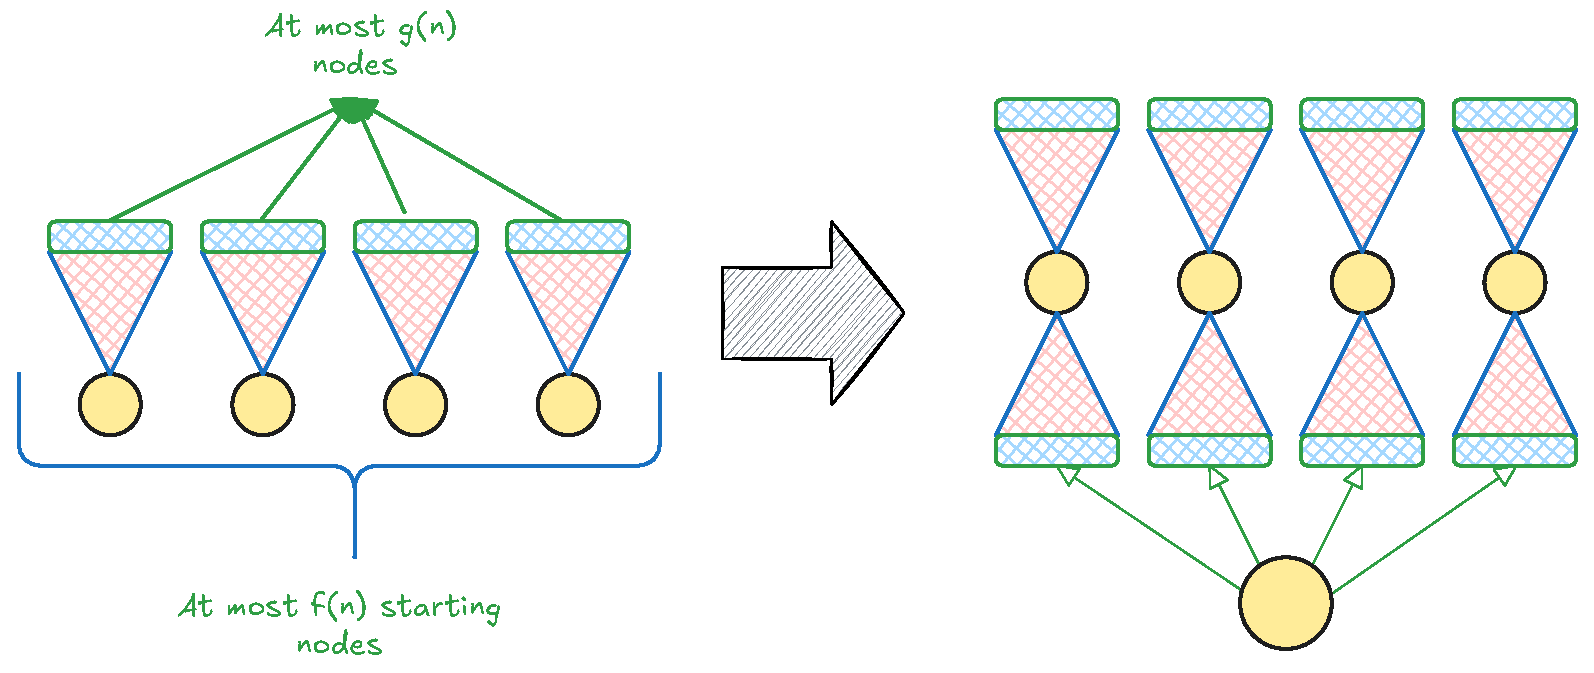
\includegraphics[width=0.5\textwidth]{Chapter3/unbalanced-multi-source.pdf}
        \caption{\textit{PolyS-Unbalanced} transformation to \textit{Unbalanced}}
        \label{fig:unbalanced-ms-trans}
    \end{figure}
\end{proof}